\section{Deployment}\label{sec:03_depl}
% Explain section
This section explains the deployment of the application.
% Requirements
The only requirement to run this application is to have tomcat 9 installed.
% Process Fig
\Fig{fig:subsubsec:03_depl_process} illustrates the process of deploying the \path{parliament.war} file using \textit{Tomcat}.
\begin{figure}[h]
\centering
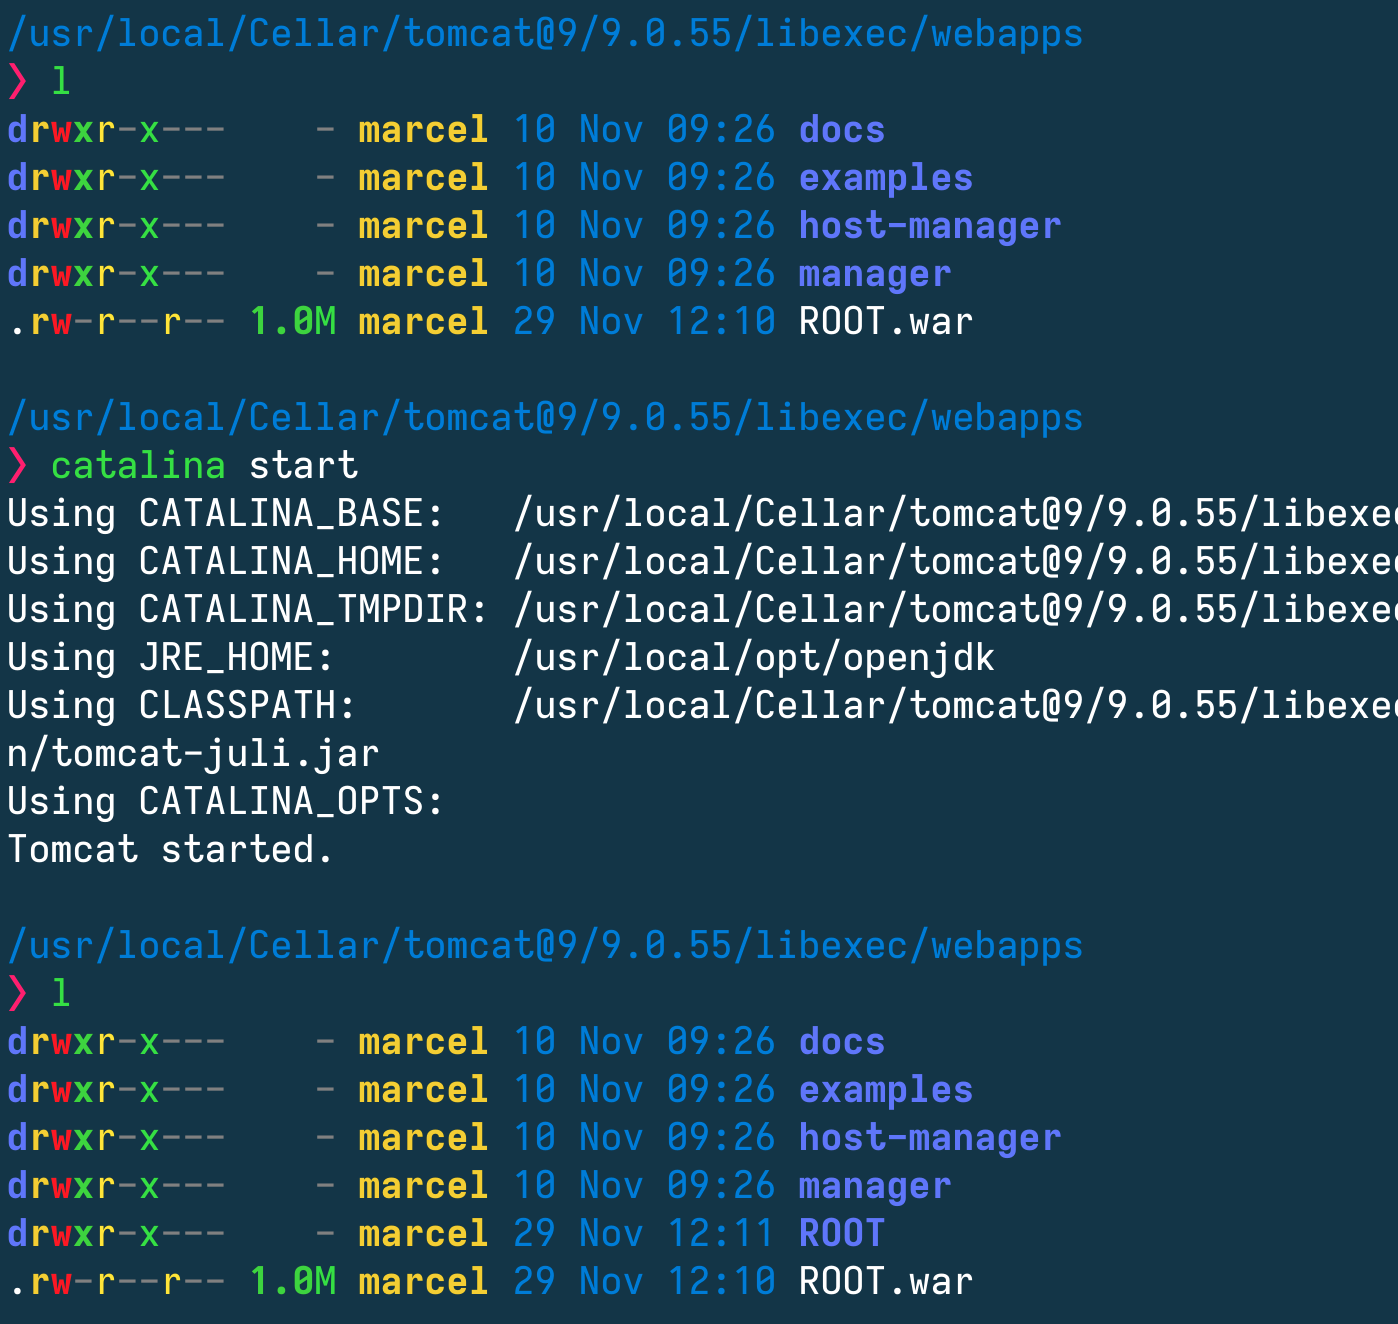
\includegraphics[scale=0.5]{images/03_depl/process}
\caption{Deployment process using \texttt{ROOT.war}}
\label{fig:subsubsec:03_depl_process}
\end{figure}

\paragraph{1.}
The first step, is to copy the \path{parliament.war} file to the \path{webapps/} folder of the \textit{Tomcat} installation.\newline
This can be done using \texttt{\$ cp parliament.war TOMCAT\_DIRECTORY/webapps}.

\paragraph{2.}
Next, the remaining step is to start the \textit{Tomcat} server using \texttt{\$ catalina start}. Tomcat will automatically extract the \path{parliament.war} to a directory called \path{parliament/}.

\paragraph{3.}
After that, the application is available via \url{http://localhost:8080/parliament/}. \Fig{fig:subsubsec:03_depl_list} shows the detail page, and \Fig{fig:subsubsec:03_depl_detail} shows the detail page of one parliament member using Firefox.

\newpage

% List page Fig
\begin{figure}[h]
\centering

\includegraphics[scale=1]{images/03_depl/member-list}
\caption{List page}
\label{fig:subsubsec:03_depl_list}
\end{figure}

\newpage

% Detail Fig
\begin{figure}[h]
\centering
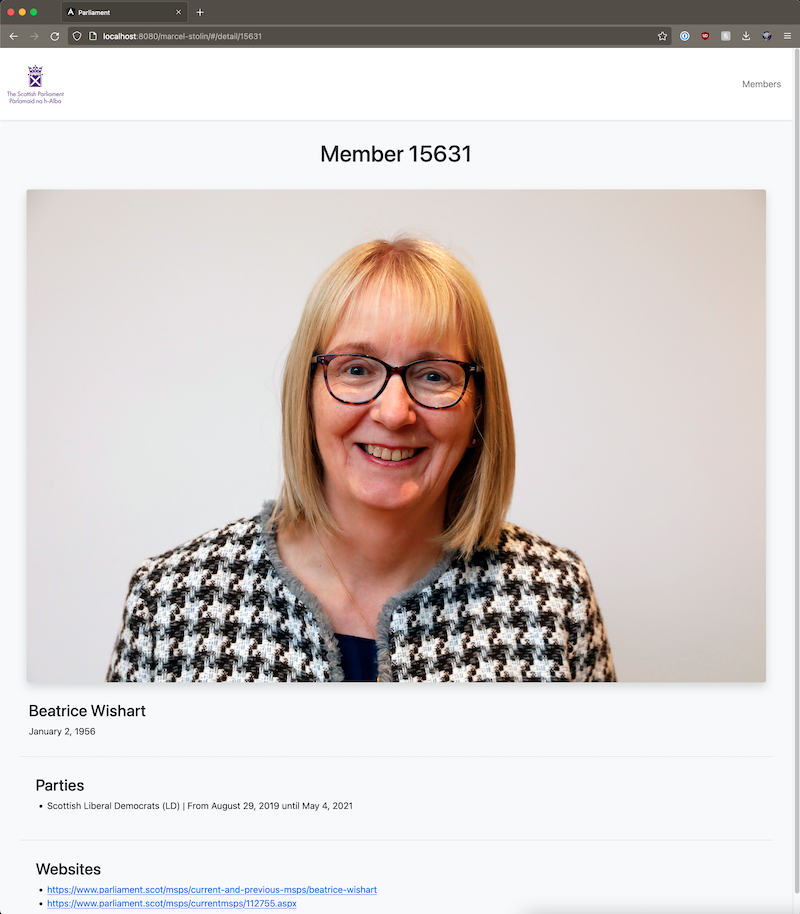
\includegraphics[scale=1]{images/03_depl/member-detail}
\caption{Detail page}
\label{fig:subsubsec:03_depl_detail}
\end{figure}
\newpage
